\chapter{Experimental Results}
\section{Imaging live cells}
For the study described in \textbf{Paper I} we used cells of two species of cyanobacteria: \textit{Cyanobium gracile} and \textit{Synechococcus elongatus}. Cyanobacteria are photosynthetic bacteria that can be found in almost any habitat on earth, ranging from hot volcanic areas to cold polar ice caps, and play an important role in the global carbon and nitrogen cycle. In a 25 day cycle an algal bloom of 1000 $km^2$ can sequester around 22,000 tonnes of atmospheric carbon into organic carbon before an infection by cyanophages cause the bloom to collapse \cite{Lehahn2014}.
 
\textit{Cyanobium gracile} cells were selected for this experiment because of their small size and their robustness with respect to the injection procedure. Single \textit{C. gracile} and \textit{S. elongatus} cells have an oval-to-cylindrical shape, and vary in size between 0.25-0.4 $\mu$m in diameter and 0.4-4.0 $\mu$m in length \cite{Komarek1999}. Cells divide symmetrically by binary fission. The two daughter cells separate from each other after reaching the size and shape of the mother cell \cite{Bazire1988}. We used non-synchronised cell cultures undergoing active growth, which means our sample contained cells in various stages of their cell cycle. 

%\subsection{Data Collection}
The experiments described in \textbf{Paper I} were carried out at the atomic, molecular, and optical science (AMO) endstation at LCLS \cite{Bostedt2013}, at a photon energy of 512 eV (corresponding to a wavelength of 2.40 nm) and 1100 eV (1.13 nm). Figure \ref{fig:experimental_geometry} shows the arrangement of the experiment. The length of the photon bunch was about 70 fs. Far-field diffraction patterns were recorded on a pair of pnCCD detectors \cite{Struder2010} in the CFEL-ASG Multi Purpose (CAMP) instrument \cite{Struder2010}. The detectors were place at 741 mm downstream from the intersection between the X-ray beam and the stream of sample. The detector read-out rate matched the 120 Hz repetition rate of the LCLS. 

We collected diffraction patterns of \textit{C. gracile} cells for an hour at a hit ratio of 43\%. The strongest 7,500 hits were selected for further analysis, using the Cheetah software package \cite{Barty2014}. The linear sampling ratio of the particle was around 20-fold, which allowed direct phase recovery from the measured intensity patterns. Phase retrieval was not a trivial problem because strong hits saturated the detectors at low diffraction angles. As a compromise, we manually selected medium-strong hits, which contained either no, or only few saturated pixels, while still providing scattered signal to reasonably high resolution. Missing mode analysis revealed no unconstrained modes for all reconstructed cells presented in \textbf{Paper I}. 

Phases were retrieved using the Hawk software package \cite{Maia2010}. For each pattern 400 reconstructions were made, each starting from different random initial phases. These reconstructions consisted of 5000 iterations with the RAAR algorithm \cite{Luke2005}, using a Shrinkwrap algorithm \cite{Marchesini2003} for support determination, and concluded with 100 iterations with the ER algorithm \cite{Fienup1978, Fienup1982}. The initial and final support sizes were manually determined. No real-value constraints were used since we anticipated the effects of absorption in the thick cells to give effects similar to a phase object. 

\begin{figure}[!ht]
	\centering 
		\includegraphics[width=120mm]{FF.png}
	\caption{Diffraction patterns and reconstructed electron densities for live C. gracile cells. The cells were alive when the femtosecond pulse traversed them but exploded some picoseconds later. Photon energy: 517 eV (water window), sample-to-detector distance: 740 mm. The total number of scattered photons in the diffractions patterns varies between 0.5 and 5 million. Each reconstructed image is the average of up to 400 independent reconstructions. Resolution was estimated from the phase retrieval transfer function. White circles in the reconstructions indicate the resolution relative to the object size. Feature smaller than the circle should not be interpreted as sample features. Reconstructions are normalized, where dark blue is 0 density and dark red is the most dense part of the cell.The cells are sorted according to cell size. Synthetic X-ray Nomarski images were calculated from the complex-valued reconstructions to show the reconstructed phase shift properties of the object together with its density.}\label{fig:Reconstructions}
\end{figure}

Figure \ref{fig:Reconstructions} shows the reconstructed exit wave-fronts for six \textit{C. gracile} cells together with the corresponding diffraction patterns, and a synthetic Nomarski image. The reconstructions represent 2D projections of the electron density of the cells. The images show the expected morphologies of cells during division \cite{Komarek1999,Bazire1988}. The resolution of each reconstruction is indicated by the size of the round white dot. This means that features smaller than the dot were not recovery reproducibly and should not be interpreted as features of the sample.

\begin{figure}[!ht]
	\centering 
		\includegraphics[width=120mm]{prtf.png}
	\caption{Image resolution of the reconstruction. For each reconstruction shown in Fig. \ref{fig:Reconstructions}, the corresponding PRTF is shown. Resolution is determined as the first time the PRTF function drops below 1/e \cite{Seibert2011}. The white dot in the reconstruction has the size of the resolution determined from the PRTF.}
	\label{fig:PRTF}
\end{figure}

The resolution of the reconstructions were estimated from the PRTF (See Figure \ref{fig:PRTF}), using the 1/e threshold. Before calculating the PRTF and averaging the repeated reconstructions we removed outliers between the reconstructions by applying a threshold to the Fourier error. Clustering validates the results from using a threshold on the Fourier error and the real-space error. On average the main cluster contained about 370 out of 400 reconstructions (93\%), except for one case where only 96 reconstructions formed the biggest cluster (Figure \ref{fig:Clustering}). That the main cluster often incorporates most reconstructions, and has the lowest error scores made us believe that the average image of the main cluster is likely to represent the best reconstruction minimum. 

\begin{figure}[!ht]
	\centering 
		\includegraphics[width=120mm]{Clustering.png}
	\caption{Scatter plots of the Fourier vs real-space error for each individual reconstruction for each average reconstruction shown in Fig. \ref{fig:Reconstructions}. Each cluster has its own color. The image in the top left corner is the average reconstruction of all the reconstructions selected within the blue box. The threshold for cluster selection has always been the Fourier error, which avoids selecting for similarity. }
	\label{fig:Clustering}
\end{figure}

Detector saturation limited the achievable resolution. A number of much stronger exposures than shown in Figure \ref{fig:Reconstructions} were also recorded, and in some of these exposures the diffraction signal extended to nanometer resolution. Figure \ref{fig:StrongHit} shows one such pattern for a live \textit{S. elongatus} cell at 1,100 eV photon energy. Two pnCCD detector pairs were used to record this pattern. The configuration of the central back detector in Figure \ref{fig:StrongHit} is identical to the detector to record the diffraction patterns shown in Figure \ref{fig:Reconstructions}. The front detector is the same type as the back detector but is placed at 220 mm from the interaction region. In strong exposures, a large part of the back detector was saturated, which prevented reliable phasing. The signal however extended beyond 4 nm resolution on the front detectors, which is the size of a small protein molecule. More than 58 million scattered photons were recorded on the back detectors, and 1.3 million on the front detectors. The size of the cell was derived from the autocorrelation, shown in the boxed panel in the middle of Figure \ref{fig:StrongHit}. 

\begin{figure}[!ht]
	\centering 
		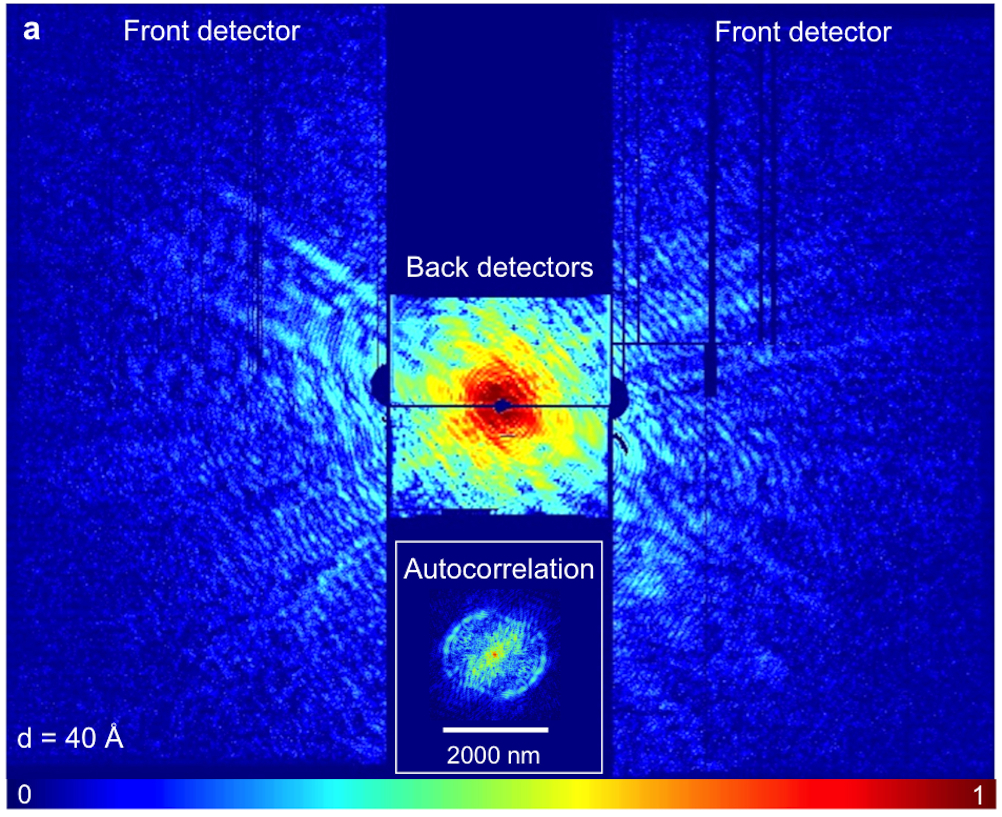
\includegraphics[width=100mm]{StrongHit.png}
	\caption{Combined diffraction signal of front and back detector. In strong hits the scattered signal from a micron-sized \textit{S. elongatus} cell extends to 4 nm full-period resolution. The size of a small molecule is 4 nm. The cell was alive during the exposure. The central area of the diffraction pattern is saturated, which prevented image reconstruction. The autocorrelation, shown in the central box, indicates the shape of the imaged cell.}\label{fig:StrongHit}
\end{figure}

\section{Data Deposition}
The ability to record millions of diffraction patterns in a day at X-ray free-electron lasers (XFELs) opens up new opportunities for experiments on cells. The massive amount of data will represent more than just individual projection images of cells. There is however a need to develop algorithms to create abstract models of cells from the data. With so many images per day, even statistically rare events could be pinpointed and studied. XFEL beam time is scarce nonetheless, and many researchers have limited access to experimental XFEL data. To aid the development of algorithms that can interpret the wealth of diffraction data we have released the data sets used in the cell study (\textbf{Paper II}). We deposited both raw and pre-processed data at the Coherent X-ray Imaging Data Bank (CXIDB) \cite{Maia2012a} (http://www.cxidb.org/id-37.html), and published a descriptor of the data that includes experimental details, as well as the structure of the deposited data, including the parameters used for data selection.

\section{RedFlamingo}

RedFlamingo has been tested on several datasets. This chapter shows four cases that illustrate different demands on the data analysis. In the first example, RedFlamingo is used for pattern classification. The main discriminatory features were size, particle elongation, and number of particles in the beam. The second example shows that RedFlamingo can be used to size particles within a wide range of sizes and shapes. The third example shows that diffraction patterns from single particles can be separated from diffraction patterns originating from multiple particles located at a distance from each other. The final example shows how the shape of elongated particles can be determined more accurately. 

\subsection{Pattern Classification of an heterogeneous RDV data set}
Rice Dwarf Virus (RDV) is the causal agent of rice dwarf disease. It can result in severe crop losses in rice and other gramineae plants in East Asian countries due to stunted growth and chlorotic specks. The structure of RDV has previously been solved to 3.5 {\AA} resolution by X-ray crystallography \cite{Nakagawa2003} (PDB 1UF2). The RDV capsid has an icosahedral symmetry, and it is approximately 72 nm in diameter across the 5-fold axis.

As part of a large international collaboration called the Single Particle Imaging initiative (SPI)\cite{Aquila2015a}, an extensive dataset of RDV hits was collected. Most diffraction patterns in this data set are not affected by detector saturation, which makes it possible to estimate the size of the icosahedral-shaped particle by determining the location of the first minima in the diffraction patterns (see Chapter 8).
RDV was classified on the size and shape of the central speckle, and the size and shape of the central term in the autocorrelation. If the central speckle and the central term of the autocorrelation are circular or only slightly elongated the particle was classified as a single particle.  

\begin{figure}[!ht]
\centering
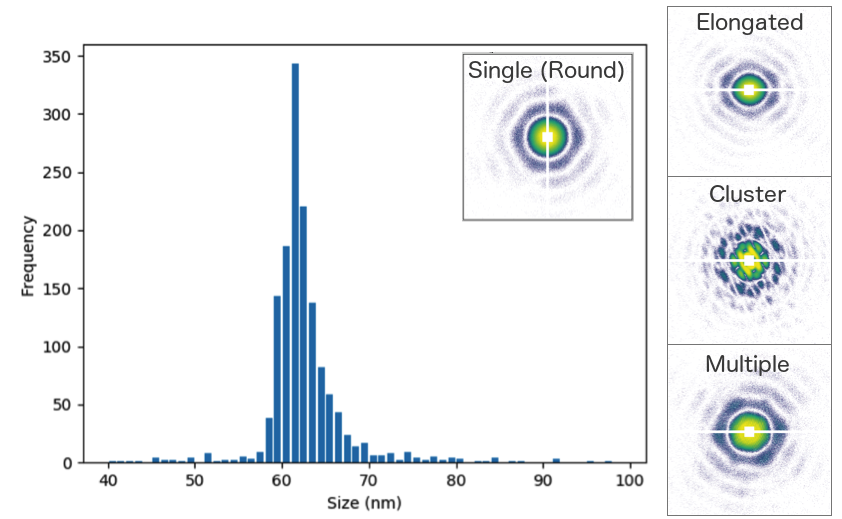
\includegraphics[width=120mm]{Chapter_09_Results_RDV.png}
\caption{Classification of particles. The size distribution of the 3608 diffraction patterns that were classified as single hits shows a peak at 63 nm. Right panels shows an  example of a diffraction pattern of each class. The gap between the two detector halves and the beam stop is masked out.}\label{fig:Classes}

\end{figure}

The diffraction patterns that have a round central speckle show features commonly associated with icosahedral particles. 

\subsection{Pattern Selection based on edges}
The second example deals with the selection of diffraction patterns based on the presence of sharp edges. The sample used was the 331-kbp chlorovirus Paramecium bursaria chlorella virus 1 (PBCV-1). PBCV-1 is the type member of the genus Chlorovirus that infects certain chlorella-like green algae from freshwater sources \cite{VanEtten2012}. It is a quasi-icosahedral particle with a diameter of 190 nm across the 5-fold axis.

In the experiment PBCV particles were injected into the XFEL focus using a GDVN. As expected for particles significantly smaller than the drop size, this resulted in a wide size distribution, of which elongation assessment showed that most particles are very round. Using the edge finding algorithm described in Chapter 8, we could find patterns that show clear features related to edges, as shown in Figure \ref{fig:PatternSelection}, separating these patterns from objects with spherical appearance.

\begin{figure}[!ht]
\centering
\includegraphics[width=120mm]{Chapter_09_Results_PBCV.png}
\caption{Measured particle size-distribution when shooting Paramecium bursaria chlorella virus 1 (PBCV-1) and xenon clusters during an X-ray holography experiment (Paper X). Sizing of hits by RedFlamingo shows a wide size distribution. Particles with a diameter of around 70 nm are likely to be Xenon-clusters. These clusters were co-injected with the PBCV particles. The peak around 170 matches the size of the PBCV particles, and the peak of particle-size 240 might be a contamination by an earlier imaged virus of approximately that size. Most particles were very spherical, but using the edge detection algorithm, patterns similar to 8.1 were selected. Six examples of such patterns are shown on the right.}\label{fig:PatternSelection}

\end{figure}


\subsection{X-ray holography on the fly - Multiple objects in the X-ray focus}

I participated in an experiment at the LCLS to capture holographic images of viruses, using two injectors simultaneously to shoot virus particles and reference objects into the X-ray beam. One of these injectors was our aerosol injector, used to inject virus particles into the X-ray focus. The other injector one was a xenon cluster source, used  to create a beam of reference objects. The cluster beam intersected the sample beam in the X-ray focus (\textbf{Paper X}). We used clusters of approximately 70 nm in diameter. A holographic diffraction pattern was recorded when the X-ray pulse simultaneously captured a sample particle and one or more reference objects. Such a pattern is similar to Figure 8.5. During the experiment, some of the hits came from single reference objects or sample particles, others from various combinations of these, including single and multiple sample particles, single and multiple reference objects, or any mixture of sample particles and reference objects. The various types of shots had to be sorted out and this was achieved by RedFlamingo, using the algorithm described in Chapter 8. Table 9.7 shows the results of the classification for samples varying between 70 and 2000 nm in size. 

\begin{figure}[!ht]
\centering
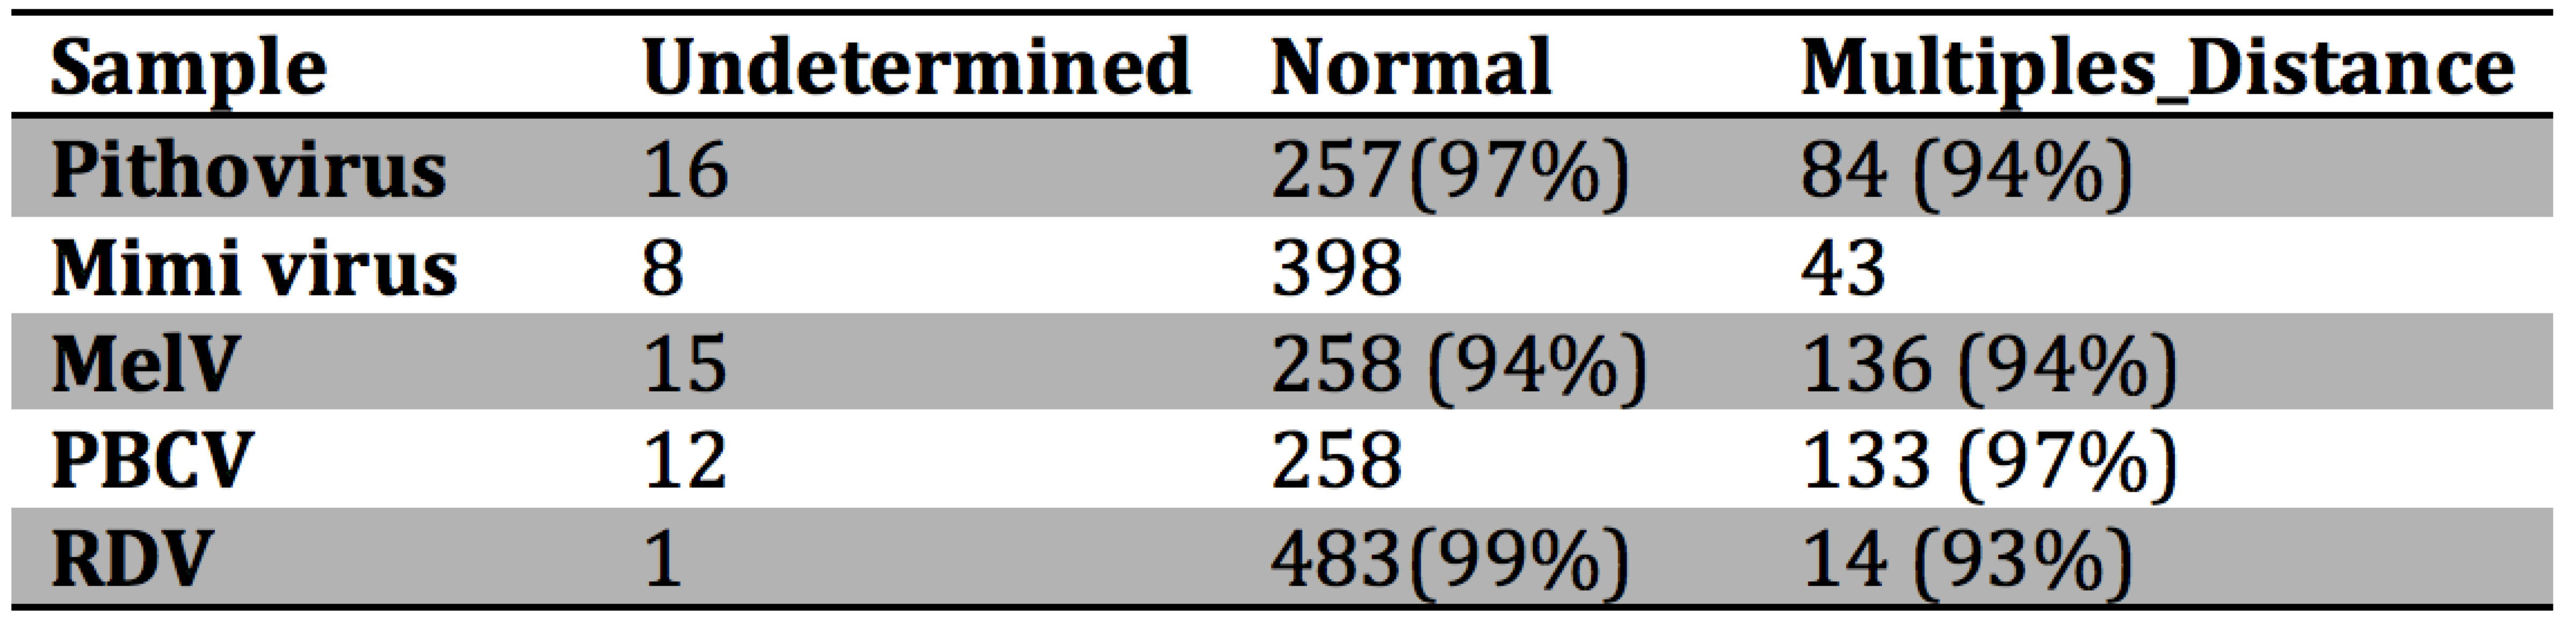
\includegraphics[width=100mm]{Chapter_09_Results_successrate.png}
\caption{Identification of multiple particles in the focus. Diffraction patterns from five different samples ranging from > 1000 nm to 70 nm in size were classified as either singles or coming from multiple particles at the same time. There are three classes: MultipleDistance, Normal, and Undetermined. Patterns with strong saturation are put in the latter class, because the autocorrelation sometimes shown strong artefacts because of it. The percentage between brackets indicates the successrate of classifying the patterns correctly in the class.}\label{fig:multiple_find}

\end{figure}

\subsection{Particle Shape Assessment}

\textit{Pithovirus sibericum} is a 30,000 year-old giant virus (about 500 nm x 2000 nm) from the Siberian permafrost and its shape resembles a “pithos”, i.e. a large amphora used by the ancient Greeks. We used RedFlamingo for the automated shape assessment of the elongated virus particle. Using the shape assessment algorithm of RedFlamingo illustrated by Figure8.4, we determined the shape of many particles. Figure 9.8 shows a scatter plot of the maximum and minimum size for each particle. The results show that a large fraction of the particles is roundish in shape. The size variations follow expectations. In the future this methods might find itself useful for the automation of the reconstruction of heterogeneous particles of unknown size, such as cells.

\begin{figure}[!ht]
\centering
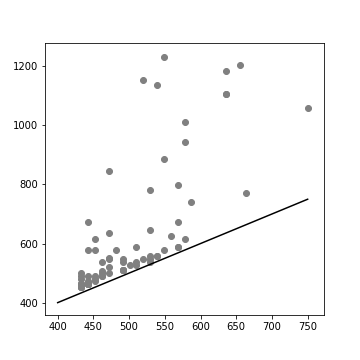
\includegraphics[width=100mm]{Chapter_09_Results_Refined_Sizing.png}
\caption{Scatter plot of the minium size of the particle vs. the maximum size of a particle, derived from the filtered autocorrelation. }\label{fig:majorminor}

\end{figure}



%\section{Software}

